\chapter{Le modèle}

\lettrine{O}{n} s'intéresse ici aux différentes approches possibles pour modéliser le système manguier~--~cécidomyies des fleurs. 
Il y a dans la littérature quelques modèles relatifs aux manguiers et aux cécidomyies.
% On décrira la solution retenue ainsi que les hypothèses faites.

Concernant la modélisation en rapport avec le manguier, on peut citer le modèle \emph{Virtual Mango} développé par \citet{fred}.
C'est un modèle qui simule le développement architectural du manguier, ainsi que la croissance et les différents stades phénologiques des unités de croissance et des inflorescences et la croissance des fruits.
Le modèle ne prend cependant pas en compte l'impact des ravageurs sur le développement de l'arbre et sa production.

Concernant la modélisation en rapport avec les cécidomyies des fleurs, on peut noter l'existence d'un modèle de colonisation d'un verger par les cécidomyies \citep{paul}. 
Les données utilisées proviennent d'une expérimentation menée sur un verger entièrement bâché. 
C'est un modèle stochastique et spatialisé qui prend en compte l'arrivée des femelles sur le verger, leurs pontes d'œufs dans les inflorescences, le développement de ces derniers jusqu'au troisième stade de développement larvaire et enfin l'éjection des larves des inflorescences.
Cependant, le fait que le verger modélisé est entièrement bâché implique l'abscence de cycle de développement complet pour les cécidomyies à l'intérieur du verger ainsi que l'absence d'émergence de cécidomyies issues de la diapause.

On choisira ici l'approche amorcée par \citet{laurie}, qui propose une modélisation non spatialisée du verger expérimental considérant l'infestation du verger par des femelles exogènes et la reproduction endogène, tout en prenant en compte les différentes modalités de couverture du sol.
L'objectif sera de simuler les dynamiques de larves à l'échelle de la sous-parcelle en fonction du nombre d'inflorescences présentes.

\section{Approche retenue et hypothèses}

L'approche retenue se veut simple.
On considèrera les populations (de cécidomyies et d'inflorescences vivantes) dans chaque sous-parcelle et non les individus.
Concrètement, cela veut dire que l'on ne considèrera que les nombres totaux d'inflorescences vivantes et de cécidomyies qu'il y a chaque jour dans chaque sous-parcelle.
Par ailleurs, la période considérée est la saison de floraison et le modèle n'est pas pluriannuel.

Les hypothèses sur les processus biologiques qui régissent le système, que nous faisons, sont :
\begin{itemize}
 \item la modalité de couverture du sol n'influe pas sur le développement et la phénologie du manguier, elle n'influe pas non plus sur le déplacement des cécidomyies ;
 \item la durée de vie des femelles n'est que d'un jour, et il correspond au jour de la ponte ;
 \item aucune cécidomyie (larve ou adulte) ne rentre dans le sol ou ne sort du sol pour la sous-parcelle avec un paillage synthétique ;
 \item il y a un taux de mortalité pour larves lorsqu'elle rentrent ou et les adultes lorsqu'ils sortent du sol, et ce taux est différent entre l'enherbement ras et l'enherbement haut ;
 \item les larves qui n'entrent pas en pupaison (soit qui meurent, soit qui rentrent en diapause) sont exclues du système ;
 \item la probabilité d'entrer en pupaison dépend de la température ;
 \item la quantité de cécidomyies en diapause est la même pour les trois sous-parcelles;
 \item un individu qui émerge dans une sous-parcelle peut se déplacer dans les autres sous-parcelles, il y a cependant un coût relatif à la distance (autrement dit, les cécidomyies préfèrent rester dans la sous-parcelle dans laquelle elles émergent, puis aller dans la sous-parcelle limitrophe plutôt que dans la troisième) ;
 \item les femelles exogènes arrivent proportionnellement aux inflorescences vivantes dans la parcelles (qui exercent un effet d'attraction) ;
 \item s’il y a significativement plus de femelles que d’inflorescences, alors elles ne peuvent pas toutes pondre ;  
 \item il y a un taux de mortalité sur les œufs pondus par les femelles, ils ne donneront pas tous des larves.
%  \item  seuls les premiers stades phénologiques de l'inflorescence sont attractifs pour les cécidomyies.
\end{itemize}

On reprend le cycle de développement de la cécidomyie présenté dans la partie~\ref{chap:cecido}, et on essaye de le traduire par des équations simples.

\section{Formalisme}

Le schéma conceptuel du modèle est visible sur la figure~\ref{fig:schema}. On le détaille ci-dessous.

Le nombre de larves est donné par 
\[
 L_{t, i} = F_{t - d_{\ell}, i} \times R \times E_0 \times \mu_{\ell}.
\]
Ici, $L_{t,i}$ désigne le nombre de larves qui s'éjectent des inflorescences à la date $t$ dans la sous-parcelle $i$, $F_{t - d_{\ell}, i}$ le nombre de femelles qu'il y avait dans la sous-parcelle $i$ une durée de développement larvaire auparavant (durée qu'il y a entre la ponte des œufs et l'apparition du dernier stade larvaire où les larves s'éjectent des inflorescences pour s'enfouir dans le sol), $R$ représente la disponibilité d'inflorescences pour les cécidomyies, $E_0$ le nombre maximal d'œufs pondus par une femelle et $\mu_{\ell}$ la probabilité de survie des œufs et larves.
En d'autres termes, cela signifie simplement que le nombre de larves à une certaine date résulte du nombre d'œufs pondus par les femelles, qui ont survécus et se sont développés --- sans oublier de prendre en compte que le développement dure quelques jours et que le nombre de femelles qui pond est conditionné à la disponibilité en ressources.

% La deuxième équation donne le nombre de femelles issues du cycle de pupaison qui émergent dans le verger :
% \begin{equation}
% F^{\text{pupe}}_{t, i} = L_{t - d_{\text{p}}, i} \times \mu_{\text{sol}} \times p_{\text{p}} \times \frac{1}{1 + \mathit{SR}}.
% \label{eq:fpupe}
% \end{equation}
% On a ici $F^{\text{pupe}}_{t}$ qui désigne le nombre de femelles issues du cycle de pupaison qui émergent à la date $t$ dans le verger, $L_{t - d_{\text{p}}}$ le nombre de larves qui sont rentrés dans le sol une durée de pupaison auparavant, $\mu_{\text{sol}}$ la probabilité pour une larve d'entrer dans le sol (qui dépend de la modalité de couverture du sol), $p_{\text{p}}$ la probabilité pour une larve d'entrer en phase de pupaison et d'y survivre et $\frac{1}{1 + \mathit{SR}}$ la proportion de larves qui se transforment en femelles (les mâles ne pondant pas, ils ne nous intéressent pas).
% Cela signifie les femelles issues de la phase de pupaison qui émergent à une certaine date correspond au nombre de larves qui ont réussies à pénétrer dans le sol, qui sont entrées en pupaison, se sont transformées en cécidomyies, ont survécues puis ont émergées --- en prenant en compte la durée de développement et la proportion de femelles chez les cécidomyies.


Dans l'équation ci-dessus, le coefficient $R$ est donné par
\[
R = \min\!\left\{1, \frac{k I_{t, i}}{ F_{t, i}} \right\}\!.
\]
Ce coefficient traduit la disponibilité en ressources pour les cécidomyies, c'est-à-dire que lorsqu'il n'y a pas suffisament d'inflorescences dans le verger par rapport au nombre de femelles, alors toutes les femelles ne peuvent pas pondre.
Il vaut 1 lorsque toutes les cécidomyies femelles peuvent pondrent ; il est compris entre 0 et 1 lorsque certaines cécidomyies femelles ne peuvent pas pondre.
Ce coefficient $R$ dépend du paramètre $k$ qui indique combien de femelles peut acceuillir une inflorescence chaque jour.

Toujours dans l'équation donnant le nombre de larves, on peut noter que le nombre de femelles présente dans la sous-parcelle $i$ au jour $t$ est donné par
\[
F_{t, i} = F^{\text{endo}}_{t, i\rightarrow i} + F^{\text{endo}}_{t, (j,k)\rightarrow i} + F^{\text{exo}}_{t, i}\!,
\]
où $F^{\text{endo}}_{t, i\rightarrow i}$ sont les femelles qui émergent dans la sous-parcelle $i$ et qui y restent, $F^{\text{endo}}_{t, (j,k)\rightarrow i}$ sont les femelles qui ont émergées dans les sous-parcelles $j$ et $k$ et qui viennent dans la sous-parcelle $i$, $F^{\text{exo}}_{t, i}$ sont les femelles exogènes à la parcelle qui viennent dans la sous-parcelle $i$.
Et le nombre de femelles exogènes est déterminé par
\[
F^{\text{exo}}_{t, i} = \gamma \times I_{t, i},
\]
avec $\gamma$ à déterminer.
Il y a aussi des échanges, entre les différentes sous-parcelles, de femelles qui ont émergées dans la parcelle.
Ainsi, le nombre de femelles qui ont émergées dans la sous-parcelle $i$ et qui vont dans la sous-parcelle $j$ est donné par
\[
F_{t, i \rightarrow j}^{\text{endo}} = \frac{I_{t, j} \times p_{\text{m}}^{\delta(i, j)}}{\sum_{n\in \{i,j,k\}} I_{t, n} \times p_{\text{m}}^{\delta(i, n)}},
\]
où $p_{\text{m}} \in [0; 1]$ et $\delta(i, n) =
\begin{cases}
0 & \text{ si } i=n \text{ (même sous-parcelle),}\\
1 & \text{ si $i$ et $n$ sont des sous-parcelles limitrophes,}\\
2 & \text{ si $i$ et $n$ sous-parcelles non-limitrophes.}\\
\end{cases}$\\
Le paramètre $p_{\text{m}}$ traduit l'intensité de la migration et le paramètre $\delta$ traduit «l'effet distance» (autrement dit, les cécidomyies préfèrent se déplacer le moins possible).

On peut noter que les femelles qui émergent comprennent les femelles issues de la phase de pupaison et celles issues de la sortie de diapause. Ainsi, on a
\[
F^{\text{endo}}_{t, i} = F^{\text{pupe}}_{t, i} + F^{\text{diap}}_{t,i},
\]
avec
\[
F^{\text{pupe}}_{t, i} = L_{t - d_{\text{p}}, i} \times \mu_{\text{sol}} \times p_{\text{p}} \times \frac{1}{1 + \mathit{SR}}.
\]
On a ici $F^{\text{pupe}}_{t, i}$ qui désigne le nombre de femelles issues du cycle de développement et qui émergent des pupes présentent dans le sol de la sous-parcelle $i$ à la date $t$, $L_{t - d_{\text{p}}, i}$ le nombre de larves qui sont rentrés dans le sol de la sous-parcelle $i$ une durée de pupaison auparavant, $\mu_{\text{sol}}$ la probabilité pour une larve d'entrer dans le sol (qui dépend de la modalité de couverture du sol), $p_{\text{p}}$ la probabilité pour une larve d'entrer en phase de pupaison et d'y survivre et $\mathit{SR}$ le ratio du nombre de mâles sur le nombre de femelles. 
Ainsi, $\frac{1}{1 + \mathit{SR}}$ donne la proportion de larves qui se transforment en femelles (les mâles ne pondant pas, ils ne nous intéressent pas).
Cela signifie les femelles issues de la phase de pupaison qui émergent à une certaine date correspond au nombre de larves qui ont réussies à pénétrer dans le sol, qui sont entrées en pupaison, se sont transformées en cécidomyies, ont survécues puis ont émergées --- en prenant en compte la durée de développement et la proportion de femelles chez les cécidomyies.
Il faut cependant noter que l'on a
\[
\mu_{\text{sol}} = \mu_{\text{sol}}^1 \times \mu_{\text{sol}}^2,
\]
où $\mu_{\text{sol}}^1$ correspond à la probabilité de survie d'une larve à la modalité de couverture du sol lorsqu'elle s'enfouit dans le sol et $\mu_{\text{sol}}^2$ désigne la probabilité de survie à la modalité de couverture du sol d'une femelle qui émerge du sol.
Cette distinction est nécessaire car les femelles qui sortent de diapause ne sont impactées par la modalité de couverture du sol qu'à la sortie des femelles (les larves étant entrées dans le sol avant la mise en place du dispositif).
On posera néanmoins, par souci de simplicité, $\mu_{\text{sol}}^1 = \mu_{\text{sol}}^2$.
Le nombre de femelles qui sortent de diapause est donné par 
\[
F_{t, i}^{\text{diap}} = D_{t} \times \frac{1}{1 + \mathit{SR}} \times \mu^{2}_{\text{sol}},
\]
où $D_{t}$ est le nombre de larves en diapause des années précédentes qui sort au jour $t$.
Le stock total de larves en diapause est donné par
\[
\texttt{stock} = \sum_t D_t.
\]


%% SCHÉMA
\begin{figure}[ht]
 \centering
 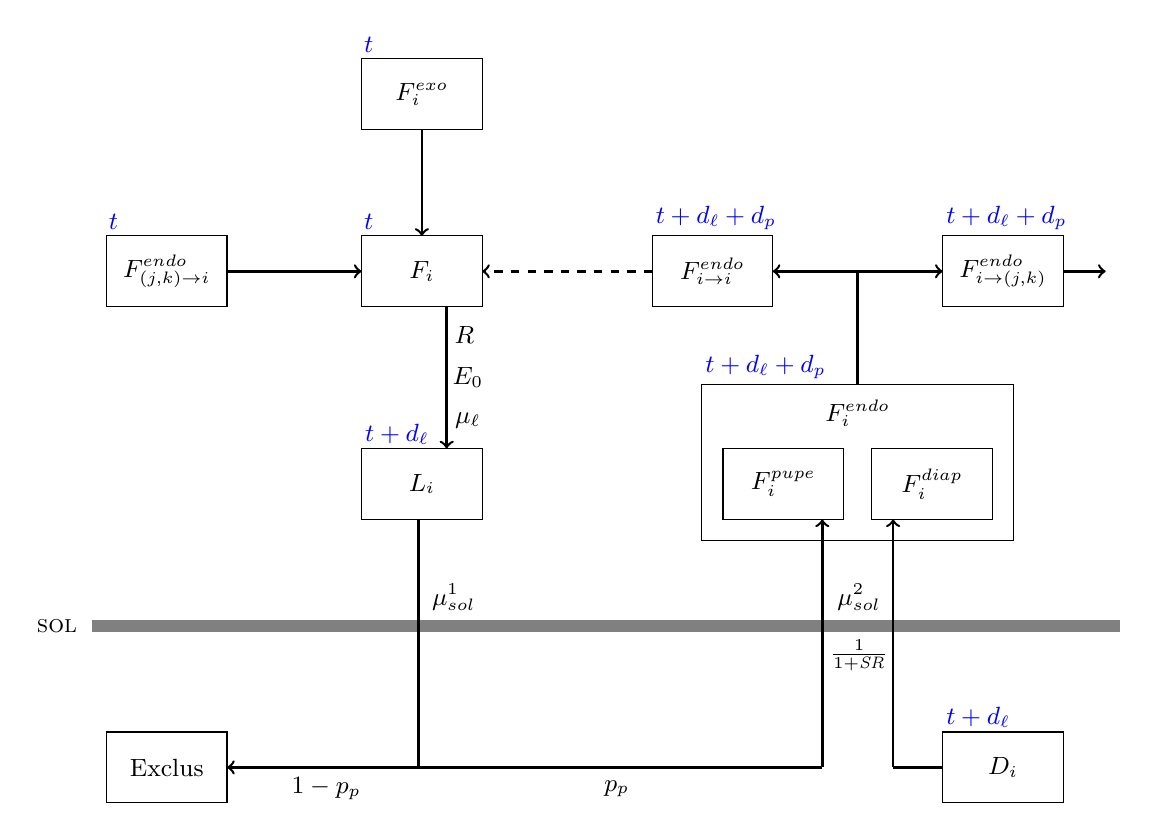
\begin{tikzpicture}[scale = 0.9]
 \draw (0, 0) node{\small \textsc{sol}};
  \draw [line width = 1.5mm, color = gray] (0.5, 0) -- (15, 0);
  % RECTANGLES
  \draw (0.7,  -1.5) rectangle (2.4,  -2.5); %diap + mort
%   \draw (8.4,  -1.5) rectangle (10.1, -2.5); % P
  \draw (12.5, -1.5) rectangle (14.2, -2.5); %Diap
  \draw (4.3,   1.5) rectangle (6,   2.5); % L
  \draw (9.4,   1.5) rectangle (11.1,  2.5); % N pupe
  \draw (11.5,  1.5) rectangle (13.2,  2.5); % N diap
  \draw (9.1,   1.2) rectangle (13.5,  3.4); % N emer
  \draw (4.3,   7) rectangle (6,   8); % N exo
  \draw (0.7,   4.5) rectangle (2.4,   5.5); % N voisins
  \draw (8.4,   4.5) rectangle (10.1,  5.5); % N endo
  \draw (12.5,  4.5) rectangle (14.2,  5.5); % N degage
  \draw (4.3,   4.5) rectangle (6, 5.5); % N
  % TEXTES CASES
  \draw (1.55, -2) node {\small Exclus};
  \draw (1.55,  5) node {\small $F^\text{endo}_{(j,k) \rightarrow i}$};
  \draw (5.15,   7.5) node {\small $F^\text{exo}_{i}$};
  \draw (5.15,   2) node {\small $L_{i}$};
  \draw (5.15,   5) node {\small $F_{i}$};
  \draw (13.35, 5) node {\small $F^\text{endo}_{i\rightarrow (j,k)}$};
  \draw (9.25,  5) node {\small $F^\text{endo}_{i\rightarrow i}$};
%   \draw (9.25, -2) node {\small $P_{i}$};
  \draw (13.35,-2) node {\small $D_{i}$};
  \draw (12.35, 2) node {\small $F^{\text{diap}}_{i}$};
  \draw (10.25, 2) node {\small $F^{\text{pupe}}_{i}$};
  \draw (11.3,  3) node {\small $F^{\text{endo}}_{i}$};
  \draw (0.8, 5.7) node {\small $\textcolor{blue}{t}$};
  \draw (4.4, 5.7) node {\small $\textcolor{blue}{t}$};
  \draw (4.4, 8.2) node {\small $\textcolor{blue}{t}$};
  \draw (4.8, 2.7) node {\small $\textcolor{blue}{t + d_{\ell}}$};
%   \draw (8.85, -1.3) node {\small $\textcolor{blue}{t + d_{\ell}}$};
  \draw (13, -1.3) node {\small $\textcolor{blue}{t + d_{\ell}}$};
  \draw (10, 3.65) node {\small $\textcolor{blue}{t + d_{\ell} + d_{\text{p}}}$};
  \draw (9.3, 5.75) node {\small $\textcolor{blue}{t + d_{\ell} + d_{\text{p}}}$};
  \draw (13.4, 5.75) node {\small $\textcolor{blue}{t + d_{\ell} + d_{\text{p}}}$};
  % LIGNES FLECHES
  \draw [line width=0.9]     (5.1,   1.5) -- (5.1,  -2);
  \draw [->,  line width=0.9] (5.1,  -2  ) -- (2.4,  -2);
%   \draw [->,  line width=0.9] (5.1,  -2  ) -- (8.4,  -2);
\draw [line width=0.9] (5.1,  -2  ) -- (10.8,  -2);
  \draw [line width=0.9]     (10.1, -2  ) -- (10.8, -2);
  \draw [line width=0.9]     (12.5, -2  ) -- (11.8, -2);
  \draw [->,  line width=0.9] (10.8,  -2 ) -- (10.8,  1.5);
  \draw [->,  line width=0.9] (11.8,  -2 ) -- (11.8,  1.5);
  \draw [line width=0.9]     (11.3,  3.4) -- (11.3,  5);
  \draw [->,  line width=0.9] (11.3,   5 ) -- (10.1,  5);
  \draw [->,  line width=0.9] (11.3,   5 ) -- (12.5,  5);
  \draw [->,  line width=0.9] (14.2,   5 ) -- (14.8,  5);
  \draw [->,  line width=0.9, dashed] (8.4,   5) -- (6, 5);
  \draw [->,  line width=0.9] (5.5,  4.5) -- (5.5, 2.5);
  \draw [->,  line width=0.9] (5.15,   7 ) -- (5.15,  5.5);
  \draw [->,  line width=0.9] (2.4,   5 ) -- (4.3,  5);
  % PARAMÈTRES
  \draw (5.6, 0.4)   node {\small $\mu_{\text{sol}}^1$};
  \draw (11.32, 0.4) node {\small $\mu_{\text{sol}}^2$};
%   \draw (6.8, -2.3)    node {\small $p_{\text{p}}$};
\draw (7.9, -2.3)    node {\small $p_{\text{p}}$};
  \draw (3.8, -2.3)    node {\small $1-p_{\text{p}}$};
  \draw (11.32, -0.42)  node {\small $\frac{1}{1 + \mathit{SR}}$};
  \draw (5.75, 4.1)     node {\small $R$};
  \draw (5.8, 3.5)     node {\small $E_0$};
  \draw (5.8, 2.9)     node {\small $\mu_\ell$};
 \end{tikzpicture}
 \caption{Schéma conceptuel du modèle pour la sous-parcelle $i$. En bleu est visible la date, la flèche en pointillés marque une rupture du temps.}
 \label{fig:schema}
\end{figure}


Le tableau~\ref{tab:param} recense les paramètres du modèle.


    \clearpage% Flush earlier floats (otherwise order might not be correct)

    \begin{landscape}% Landscape page
\begin{table}
\caption{Les différents paramètres du modèle.}
\label{tab:param}
\centering
{
\begin{tabular}{p{2cm}p{11.9cm}p{5cm}}
\textbf{Paramètre} & \textbf{Définition} & \textbf{Valeur}\\
$\gamma$ & Paramètre régulant l'arrivée des individus exogènes au verger & Calibration\\
$p_{\text{m}}$ & Paramètre régulant l'intensité des échanges entre sous-parcelles & Calibration\\
$\mu_{\text{sol}}^1$ & Probabilité de survie des larves lorsqu'elles s'enfouissent dans le sol à la modalité de couverture du sol & Calibration\\
$\mu_{\text{sol}}^2$ & Probabilité de survie des femelles qui émergent (de pupaison ou de diapause) la modalité de couverture du sol & Calibration\\
$k$ & Paramètre quantifiant le nombre de femelles que peut acceuillir une inflorescence chaque jour & Calibration\\
\texttt{stock} & Nombre d'individus entrés en diapause les années précédentes qui émergent l'année considérée & Calibration  \\
$E_0$ & Nombre maximal d'œufs pondus par une femelle & $\sim\!150$ \citep{paul}\\
$\mu_{\ell}$ & Probabilité de survie des œufs et des larves & $\sim\!0.04$ \citep{paul}\\
$\mathit{SR}$ & \textit{Sex-ratio} & 0.5 \citep{paul}\\
$p_{\text{p}}$ & Probabilité pour une larve d'entrer en phase de pupaison et d'y survivre & $\sim\! 0.77$ \citep{pauldiap}\\
$d_{\ell}$ & Durée (en jours) de la période entre la ponte et l'appartition du troisième stade de développement larvaire & 7 à 12 \citep{paul} \\
$d_{\text{p}}$ & Durée (en jours) de la phase de pupaison & 4 à 6 \citep{paul}
\end{tabular}
}
\end{table}
    \end{landscape}

% 
% \clearpage
% 
% \section{Inflorescences}
% 
% Le modèle prendra en entrée les inflorescences.
% Il faut cependant noter qu'il ne prendra pas les inflorescences «brutes», mais des dynamiques modifiées.
% En effet, on émet également l'hypothèse que les cécidomyies n'attaquent non pas les toutes les inflorescences mais uniquement celles se situant au stades phénologiques C, D ou E.
% Ce qui correspond aux seize premiers jours de l'inflorescence.
% Pour parvenir à avoir lesdites dynamiques, on a besoin de procéder à quelques étapes intermédiaires.
% On a notamment besoin de la date de débourrements des inflorescences avant d'avoir une estimation des dynamiques voulues.
% 
% \subsection{Débourrements}
% 
%  Afin de pouvoir simuler des dynamiques d'inflorescences avec une durée de vie de seize jours, il est nécessaire d'avoir les dates de débourrements des inflorescences.
%  Dans le verger n\textdegree1, les dynamiques pour les modalités «enherbement ras» et «paillage synthétique» issues des deux jeux de données ont des dynamiques plutôt similaires ; on pourrait donc utiliser les débourrements du \emph{dataset 1} mis à l'échelle.
%  En revanche, pour la modalité «enherbement haut», on observe des dynamiques très différentes. 
%  Et comme l'on souhaite privilégier les dynamiques issues du \emph{dataset 2}, il faut procéder autrement.
%  (Il en va de même pour les modalités «enherbement ras» et «paillage synthétique» du verger n\textdegree2.)
%  
%  L'objectif est alors de simuler les dates de débourrements qui permettent de produire la dynamique d'inflorescences vivantes du \emph{dataset 2}.
%  Pour cela, on suppose que la durée de vie effective d'une inflorescence suit une loi normale.
%  On possède les durées de vies effectives dans le \emph{dataset 1}.
%  Premièrement, en fixant le risque de première espèce à $\alpha = 5\%$, un test de normalité de Shapiro--Wilk nous confirme la normalité ($p$-valeur de 0.05447, on ne rejette donc pas l'hypothèse de normalité).
%  Deuxièmement, on observe une durée de vie effective moyenne de 29 jours (avec un écart-type de 14).
%  Ainsi, il faut donc simuler des débourrements, pour que des inflorescences ayant une durée de vie qui suit une $\mathcal{N}\left( 29; 14 \right)$, donne la dynamique d'inflorescences vivantes du \emph{dataset 2}.
%  Il faut donc trouver les $B_t$ tels que 
%  \[
%  I_{t}^{2} = B_t + \sum_{j = 1}^{50} B_{t - j} \times \left( 1 - F\left( j \right) \right),  \qquad \text{ avec } B_{t} = 0 \text{ si } t \leq 0,
%  \]
%  où $F$ est la fonction de répartition d'une $\mathcal{N}\left( 29;14 \right)$.
%  
%  Par souci d'homogénéïté, on utilisera les débourrements simulés pour les trois modalités, et ce pour les deux vergers.
%  
%  
% \subsection{Dynamiques}
% 
% 
% Une fois les dates de débourrements obtenus, on peut simuler des dynamiques d'inflorescences aux stades phénologiques C, D et E.
% Ces inflorescences \emph{attractives} peuvent se calculer en utilisant la formule
% \[
% I_{t}^{a} = B_t + \sum_{t = 1}^{16} B_{t-j} \times \left( 1 - F(j) \right), \qquad \text{ avec } B_{t} = 0 \text{ si } t \leq 0. 
% \]
% Ici, $B_t$ représente toujours le nombre de débourrements à la date $t$ et $F$ la fonction de répartition d'une $\mathcal{N}\left( 29; 14 \right)$.
